\begin{figure}
    \centering
    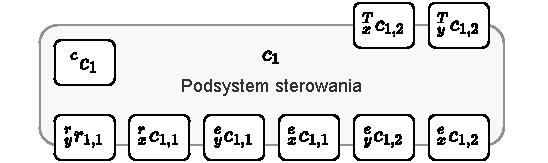
\includegraphics[width=\columnwidth]{figures/ISR-cs-model.pdf}
    \label{fig:model-cs}
    \caption{Struktura ogólna podsystemu sterowania}
\end{figure}

\begin{figure}
    \centering
    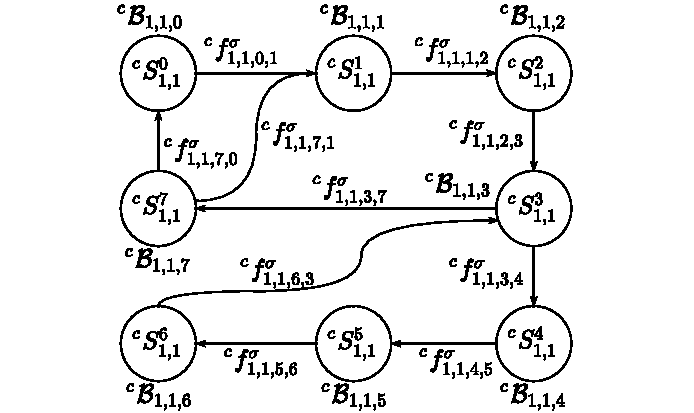
\includegraphics[width=\columnwidth]{figures/ISR-cs-behaviours.pdf}
    \label{fig:zachowania-cs}
    \caption{Automat zachowań podsystemu sterowania}
\end{figure}

Zachowania:
\begin{itemize}
    \item ${}^{c}\mathcal{B}_{1,1,0}$ - idle,
    \item ${}^{c}\mathcal{B}_{1,1,1}$ - prepare for grip,
    \item ${}^{c}\mathcal{B}_{1,1,2}$ - detect,
    \item ${}^{c}\mathcal{B}_{1,1,3}$ - grip,
    \item ${}^{c}\mathcal{B}_{1,1,4}$ - prepare for storing,
    \item ${}^{c}\mathcal{B}_{1,1,5}$ - find place for storing,
    \item ${}^{c}\mathcal{B}_{1,1,6}$ - drop in storage.
\end{itemize}